\documentclass{beamer}

\usepackage[utf8]{inputenc}
\usepackage[ngerman]{babel}
\usepackage{beamerthemeshadow}
\usepackage{calc}
\usepackage{ifthen}
\usepackage{tikz}
\usepackage{caption}
\usepackage{subcaption}
\usepackage{bchart}
\usepackage{wrapfig}

\usepackage{pgf-pie}


\newcommand{\slice}[4]{
  \pgfmathparse{0.5*#1+0.5*#2}
  \let\midangle\pgfmathresult

  % slice
  \draw[thick,fill=black!10] (0,0) -- (#1:1) arc (#1:#2:1) -- cycle;

  % outer label
  \node[label=\midangle:#4] at (\midangle:1) {};

  % inner label
  \pgfmathparse{min((#2-#1-10)/110*(-0.3),0)}
  \let\temp\pgfmathresult
  \pgfmathparse{max(\temp,-0.5) + 0.8}
  \let\innerpos\pgfmathresult
  \node at (\midangle:\innerpos) {#3};
}

\title{KMU Umweltmanagement --- Kontextmodul HS12}
\subtitle{Interdisziplinäre Projektarbeit des Kontextmoduls 1 \\ der Hochschule Luzern -- Technik und Architektur}
\author{Kontextgruppe 8}

\begin{document}

\section{Einleitung}
%\subsection{KMU Umweltmanagement}
%\frame{\frametitle{KMU Umeltmanagement\hfill{}\footnotesize HSLU -- T\&A}
% \begin{center}
% \huge
% \vfill{}
% Interdisziplinäre Projektarbeit
% \vfill{}
% Kontextmodul 1
% \vfill{}
% \normalsize
% \end{center}
% }
\maketitle

\author{Adriano Chiara}
\subsection{Begrüssung \& Programm}
\frame{\frametitle{Programm\hfill{}\footnotesize HSLU -- T\&A}
\tableofcontents

}
\subsection{Kontext}
\frame{\frametitle{Kontext, Relevanz und Auftrag\hfill{}\footnotesize HSLU -- T\&A}
% \begin{itemize}
%  \item Ressourcen
%  \item Umweltmanagement
% \end{itemize}
\begin{figure}
 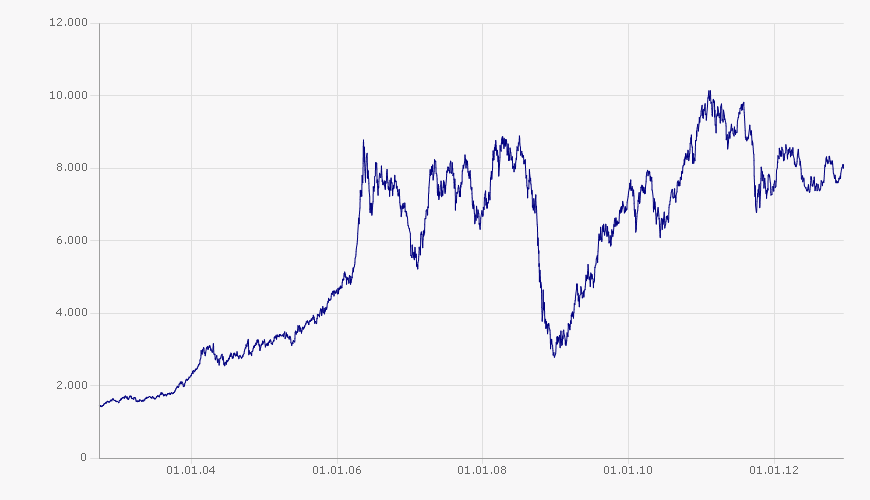
\includegraphics[width=0.9\textwidth]{kupferaktie.png}
 \caption{Kupferaktie 2004 -- 2012}
\end{figure}
}

% \begin{itemize}
%  \item Ressourcen
%  \item Umweltmanagement
% \end{itemize}


\subsection{Printprocess AG}
\frame{\frametitle{Das Unternehmen\hfill{}\footnotesize HSLU -- T\&A}


\begin{columns}
\begin{column}{5cm}
\begin{block}{Printprocess AG}
 \begin{itemize}
  \item<1> Fertigungstiefe
  \item<1> Entwicklung
  \item<1> Kunden
 \end{itemize}
\end{block}
\vspace{1cm} 
\end{column}
\begin{column}{5cm}
\begin{overprint}
\begin{figure}
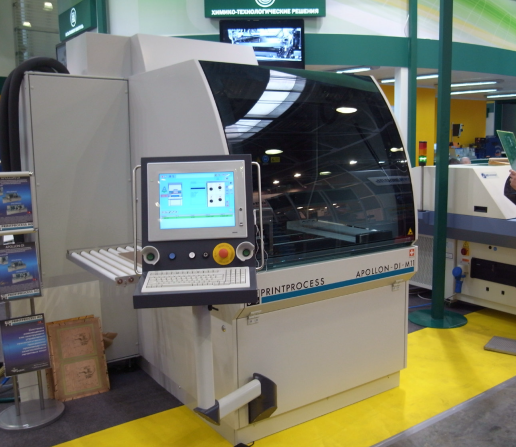
\includegraphics[scale=0.5]{ppag.png}
 \caption{Multilayergerät}
\end{figure}
\end{overprint}
\end{column}
\end{columns}
% 
% 
% \begin{itemize}
%  \item Fertigungstiefe
%  \item Entwicklung
%  \item Kunden
% \end{itemize}
% \begin{figure}
%  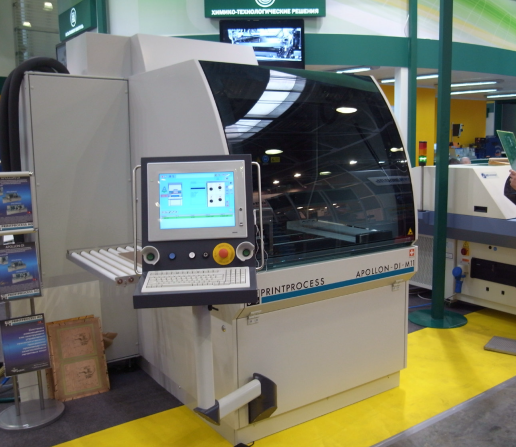
\includegraphics[width=0.4\textwidth]{ppag.png}
%  \caption{Multilayergerät}
% \end{figure}

}
\author{Ervin Mazlagic}
\section{Methode}
\subsection{Input-Output Analyse}
\frame{\frametitle{Input-Output\hfill{}\footnotesize HSLU -- T\&A}
\begin{figure}
\centering
\begin{subfigure}{0.3\textwidth}
        \begin{tikzpicture}
            \pie[text=pin, radius=1.3, rotate=330, explode ={0, 0.2}]{    67/ VP-Material,
                                           %5/ Plastik,
                                           %27/ Karton,
                                           %5/ Papier,
                                           %4/ Kupfer,
                                           %11/ Alteisen,
                                           %3/ Chrom-Nickel,
                                           %3/ Alu,
                                           33/ Metalle \& E-Schrott
                                           %31/ Altholz,
                                           %11/ E-Schrott
                                           }
        \end{tikzpicture}
        \caption{Übersicht}
\end{subfigure}
\begin{subfigure}{0.65\textwidth}
    \begin{tikzpicture}
        \pie[text=pin, radius=1.9, rotate=300, sum=32, after number=\%]{        4/ Kupfer,
                                           11/ Alteisen,
                                           3/ Chrom-Nickel,
                                           3/ Alu.,
                                           11/ E-Schrott}
    \end{tikzpicture}
    \caption{Metalle \& E-Schrott}
\end{subfigure}

\caption{Abfallaufteilung nach Gewicht}
\end{figure}
}
\subsection{Mitarbeiterumfrage}
\frame{\frametitle{Mitarbeiterumfrage\hfill{}\footnotesize HSLU -- T\&A}
\begin{figure}
\begin{bchart}[step=20,max=100,width=0.9\textwidth]
        \bcbar[text=Recycling und Abfallrennung]{91}
            \smallskip
        \bcbar[text=Arbeitsicherheit]{73}
            \smallskip
        \bcbar[text=Produkte \& Dienstleistungen]{72}
            \smallskip
        \bcbar[text=Motivation zum Umweltschutz]{63}
            \smallskip
        \bcbar[text=derzeitige Praxis ]{63}
    \end{bchart}
 \caption{Essentielle Umfragepunkte}
\end{figure}
}
\subsection{Ecomap}
\frame{\frametitle{Ecomaps\hfill{}\footnotesize HSLU -- T\&A}
% Untersuchung zu:
% \begin{itemize}
%  \item Abfall
%  \item Energie
%  \item Sicherheit
% \end{itemize}
% 
% \begin{wrapfigure}{r}{0.3\textwidth}
%   \begin{center}
%     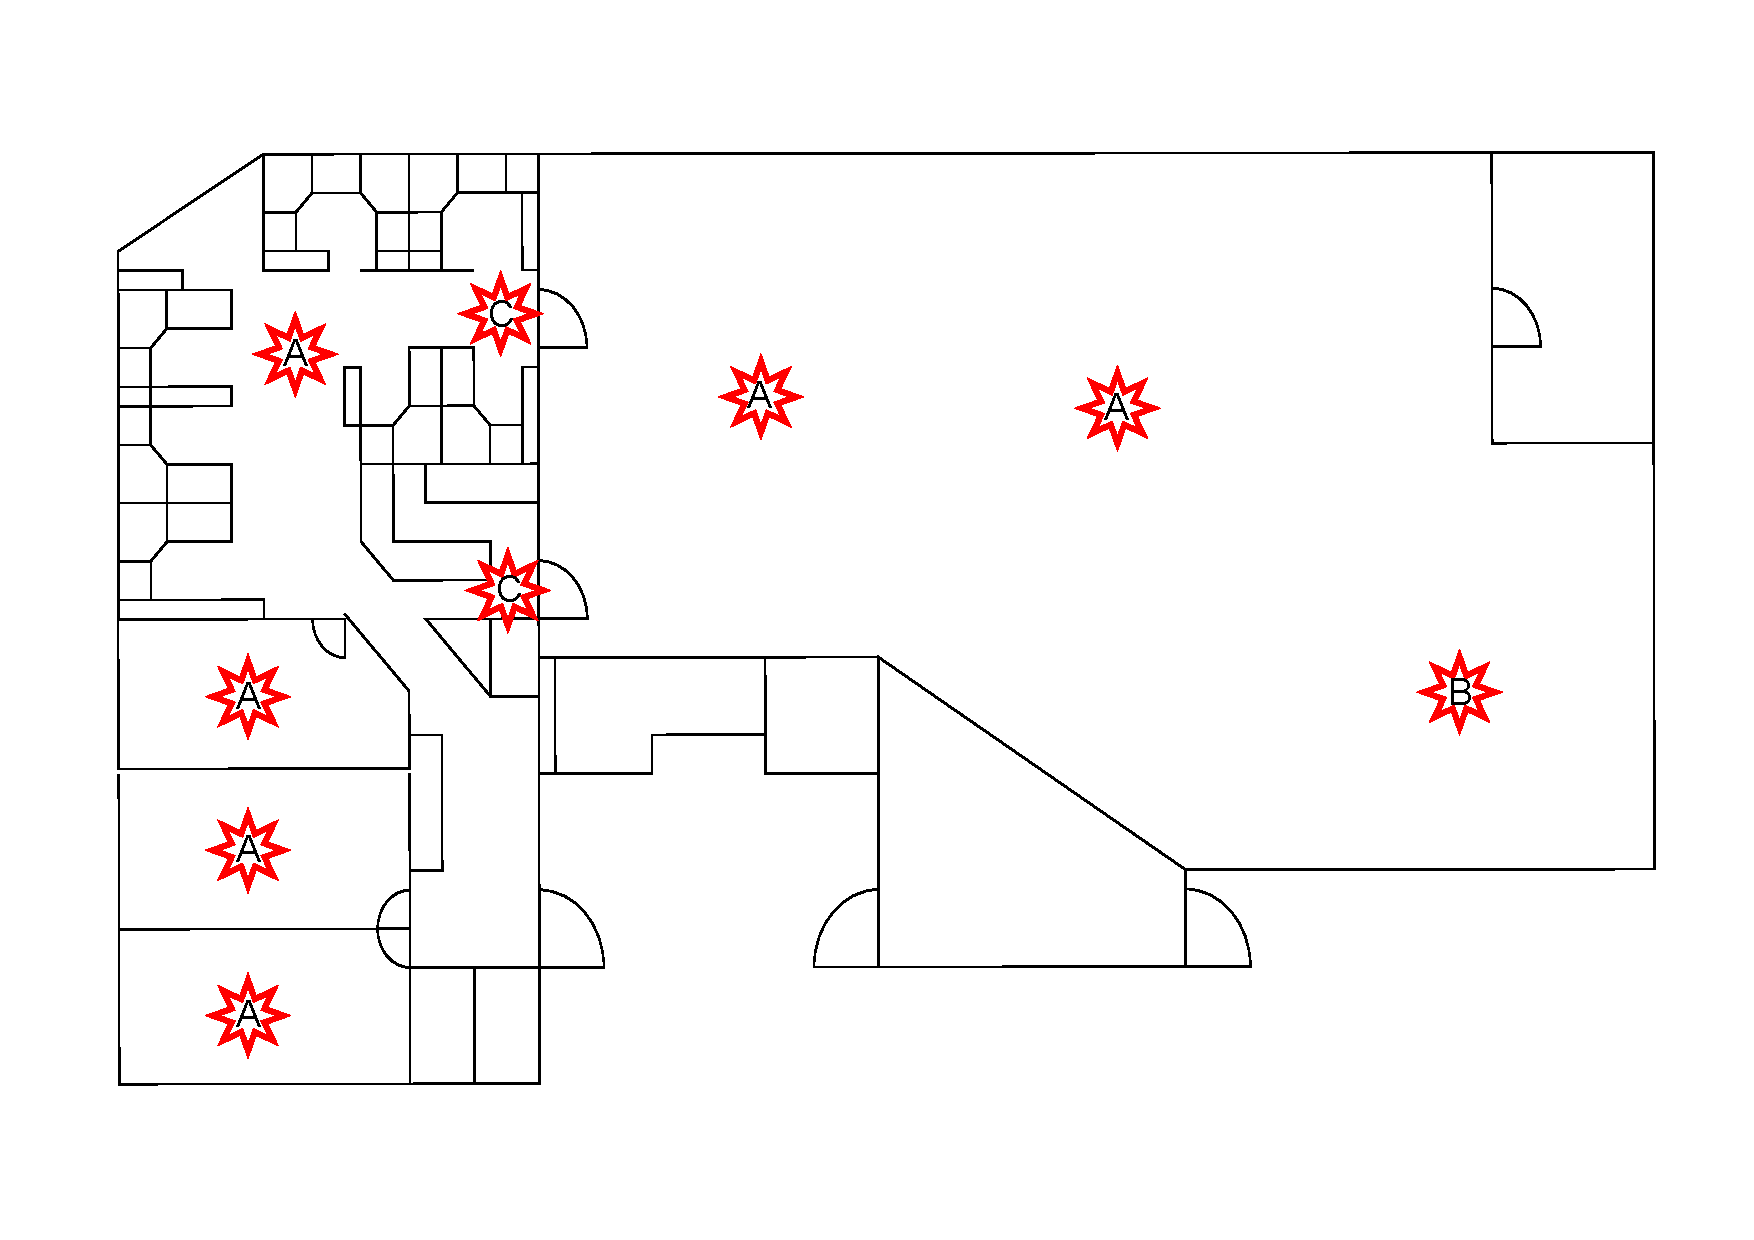
\includegraphics[width=0.5\textwidth]{ecomap.pdf}
%   \end{center}
%   \caption{Energie-Ecomap}
% \end{wrapfigure}
% 
% \begin{figure}
%  \raggedleft
%  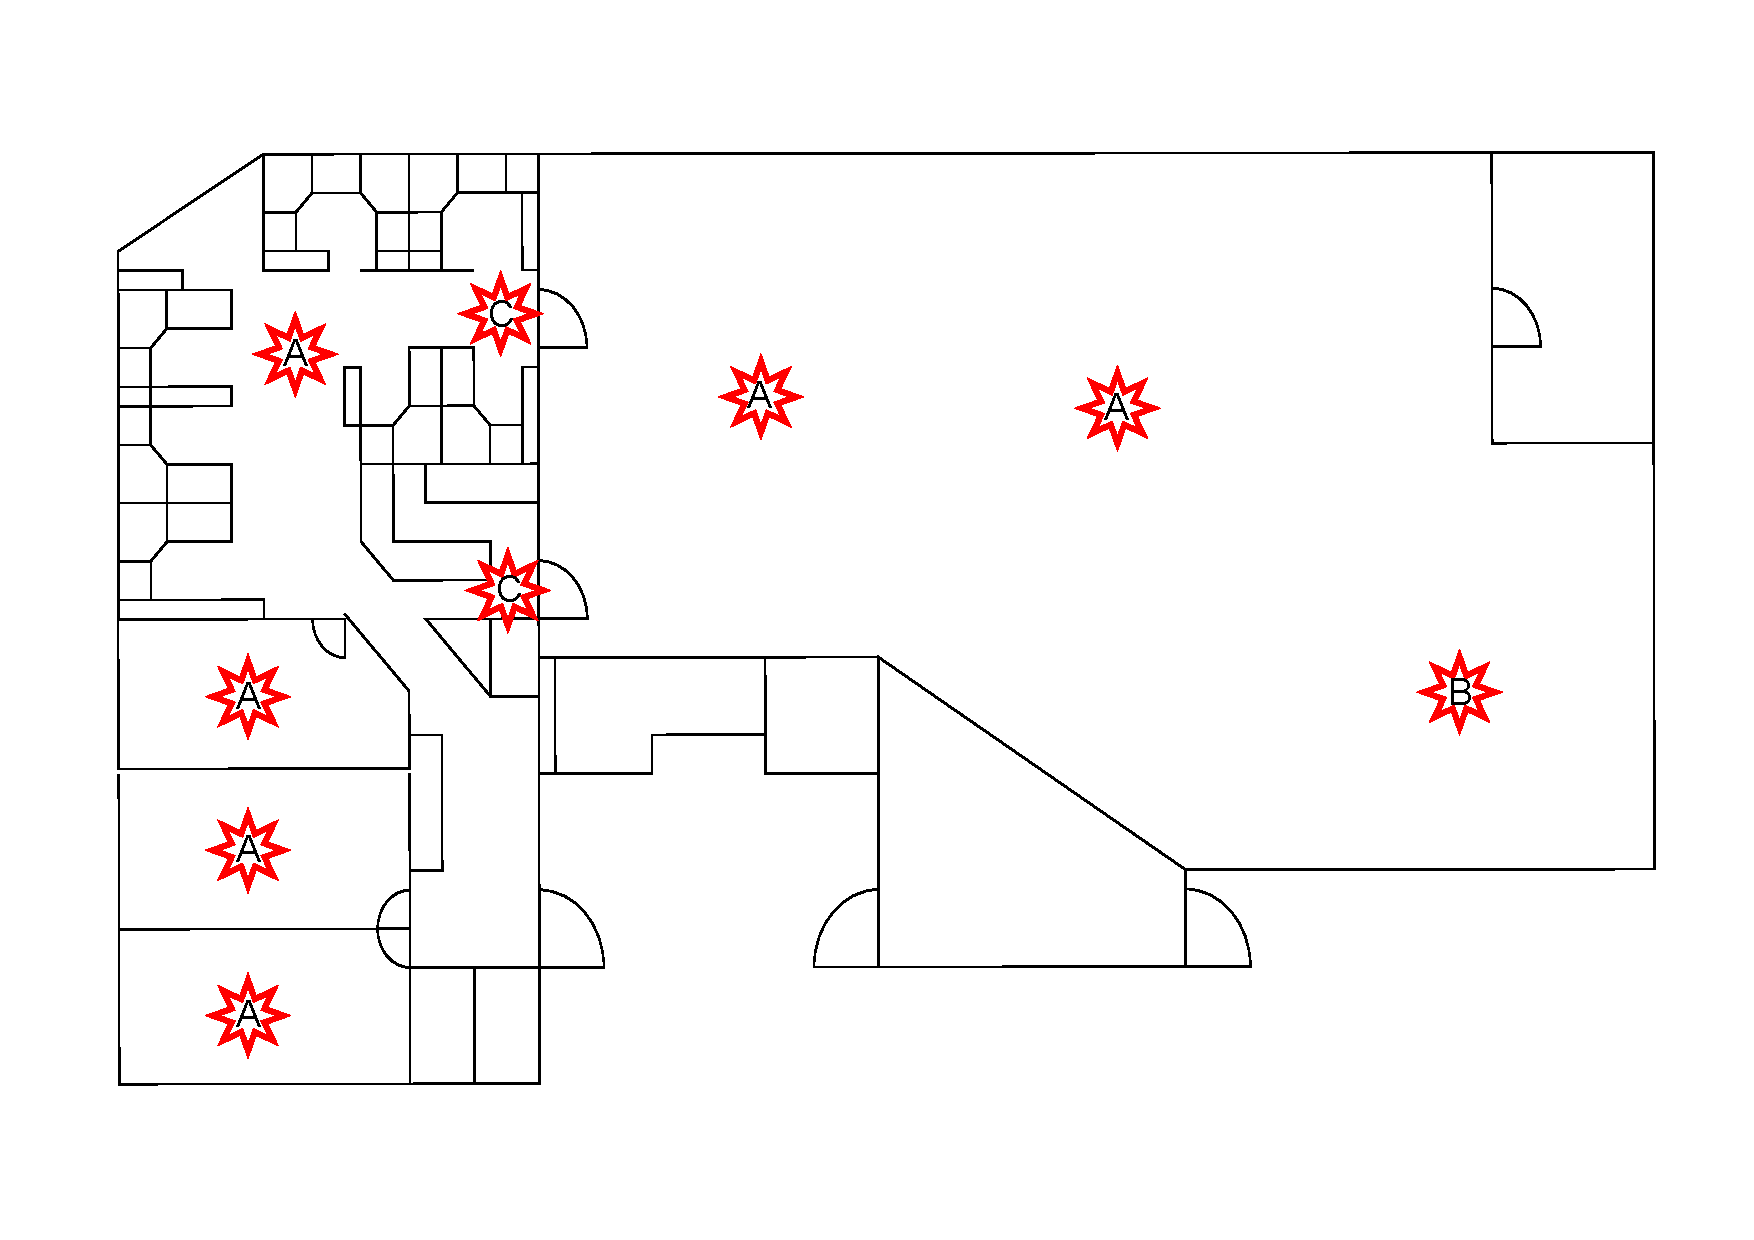
\includegraphics[width=0.5\textwidth]{ecomap.pdf} 
%  \caption{Energie-Ecomap}
% \end{figure}
\begin{columns}
\begin{column}{5cm}
\begin{block}{Untersuchung der Bereiche}
\begin{itemize}
\item<1-> Abfall
\item<2-> Energie
\item<3-> Sicherheit
\end{itemize}
\end{block}
\vspace{1cm} 
\end{column}
\begin{column}{5cm}
\begin{overprint}
\includegraphics<1>[scale=0.2, angle=270]{ecomap_abfall.pdf}
\includegraphics<2>[scale=0.2, angle=0]{ecomap_energie.pdf}
\includegraphics<3>[scale=0.2, angle=270]{ecomap_sicherheit.pdf}
\end{overprint}
\end{column}
\end{columns}
}

% \frame{\frametitle{Methodik der Analyse}
% \begin{itemize}
%  \item Input-Output Analyse
%  \item Mitarbeiterumfrage
%  \item Ecomaps
% \end{itemize}
% \begin{figure}
%  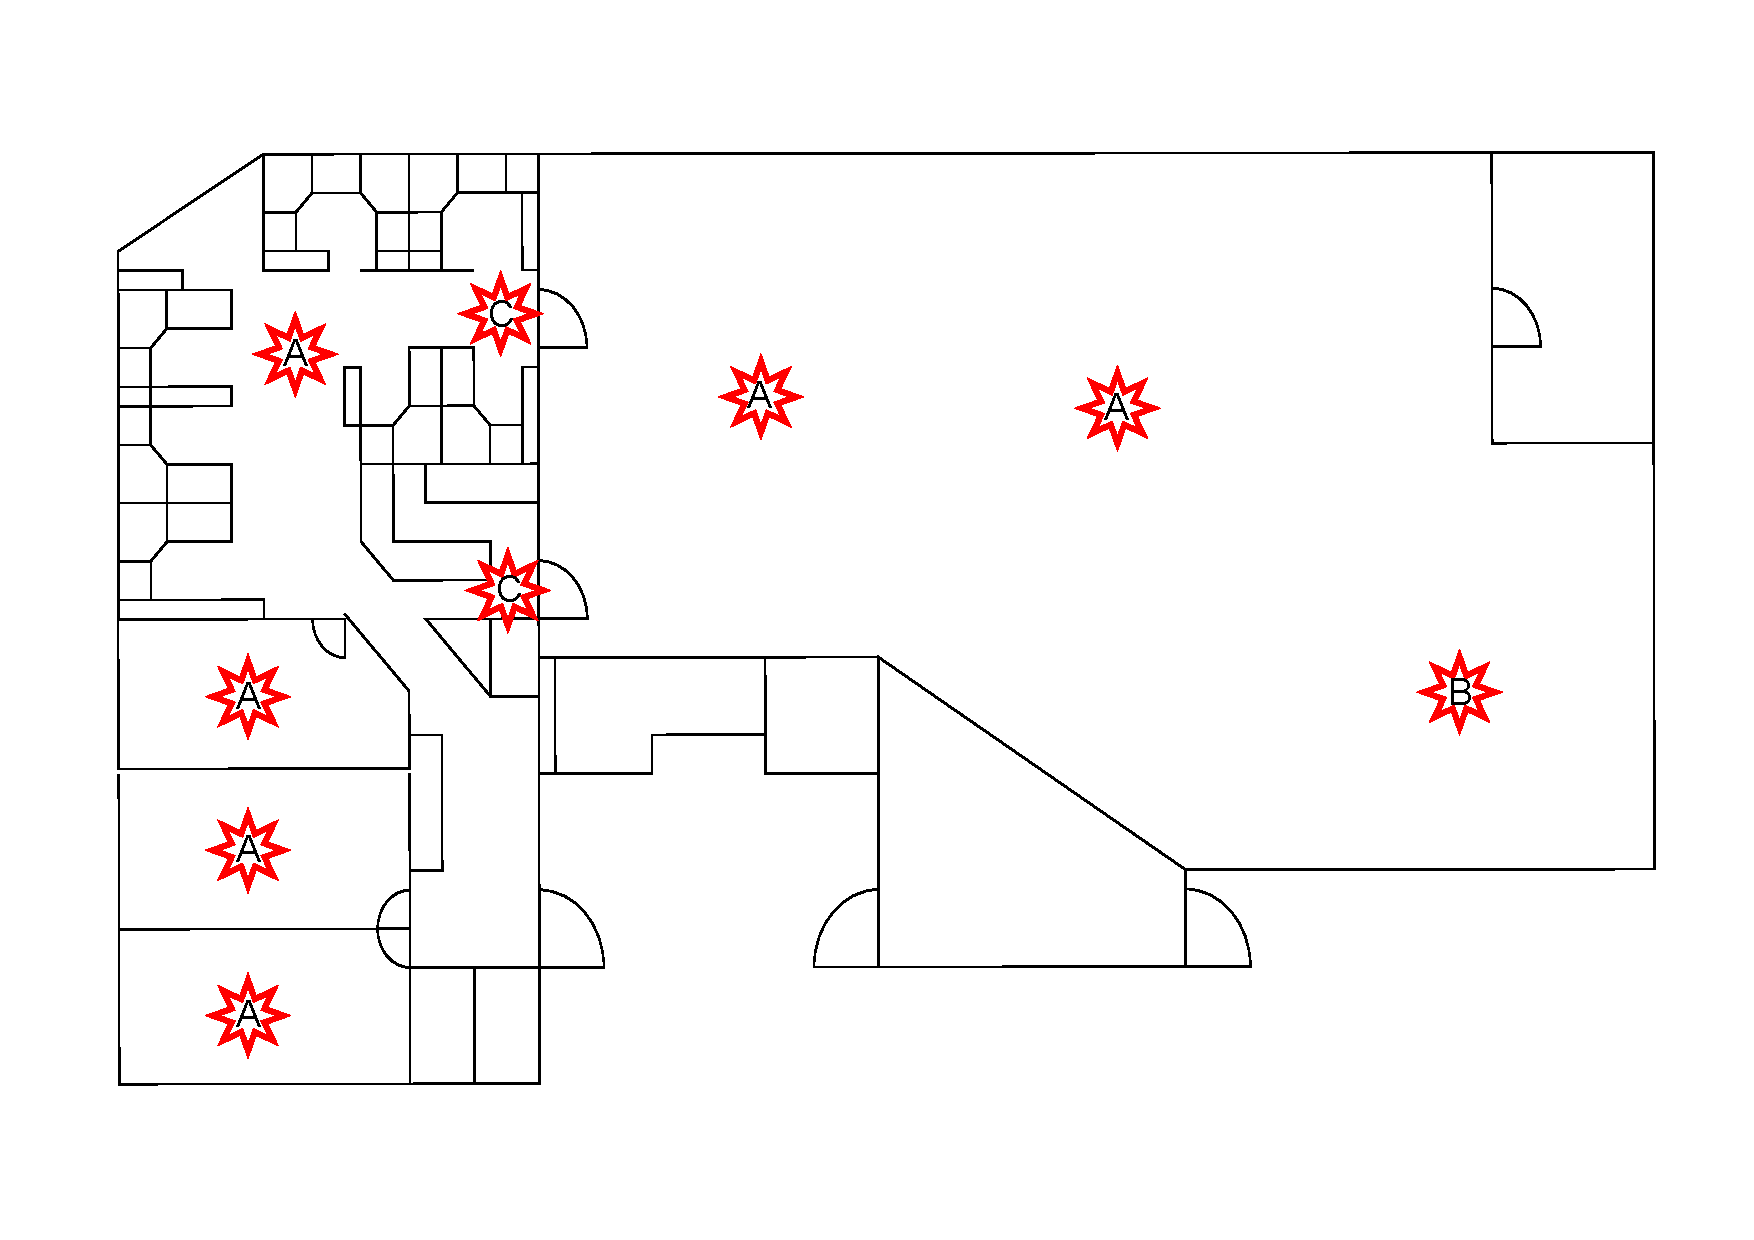
\includegraphics[width=0.5\textwidth]{ecomap.pdf}
%  \caption{Energie-Ecomap}
% \end{figure}
% }



\author{Ervin Mazlagic}
\section{Ergebnisse}
\subsection{Abfall}
\frame{\frametitle{Ecomap zum Abfall\hfill{}\footnotesize HSLU -- T\&A}

% \begin{block}{Aktuelle Lage}
% \begin{itemize}
%  \item Bestehendes Konzept übertrifft Standard
% \end{itemize}
% \end{block}
% 
% \begin{block}{Ziele}
% \begin{itemize}
%  \item Kupferanteil soll auf 33\% steigen
% \end{itemize}
% \end{block}

\begin{itemize}
 \item Bestehendes Konzept übertrifft Standard
 \item Kupferanteil soll auf $33\%$ steigen
\end{itemize}

\begin{figure}
    \begin{subfigure}{0.4\textwidth}
        \begin{tikzpicture}
            \pie[radius =1.2, pos ={0 ,0}]{25/  , 75/}
        \end{tikzpicture}
        \caption{bis 2012}
    \end{subfigure}
    \begin{subfigure}{0.4\textwidth}
        \begin{tikzpicture}
            \pie[text=legend, radius=1.2, pos ={6 ,0}]{33/ Kupfer, 67/ Elektro}
        \end{tikzpicture}
        \caption{ab 2012}
    \end{subfigure}
\caption{Elektroabfälle}
\end{figure}
}

\subsection{Energie}
\frame{\frametitle{Ecomap zur Energie\hfill{}\footnotesize HSLU -- T\&A}
\begin{block}{Aktuelle Lage}
\begin{itemize}
 \item Beleuchtung mit FL-Röhren
 \item Heizungsmanagement fehlerhaft 
 \item EVD-Geräte nicht optimiert
\end{itemize}
\end{block}

\begin{block}{Ziele}
\begin{itemize}
 \item Beleuchtung umrüsten auf LED
 \item kontrolliertes Heizen- \& Kühlen
 \item Energieoptionen der Geräte ausnutzen 
 \item Energieverbrauch jährlich um 5\% senken
\end{itemize}
\end{block}
}
\author{Adriano Chiara}
\subsection{Sicherheit}
\frame{\frametitle{Ecomap zur Sicherheit\hfill{}\footnotesize HSLU -- T\&A}

\begin{columns}
\begin{column}{5cm}
\begin{block}{Aktuelle Lage}
\begin{itemize}
 \item<1> Versperrte Fluchtwege und Notausgänge
 \item<1> Fehlende Feuerlöscher 
\end{itemize}
\end{block}
\begin{block}{Ziele}
\begin{itemize}
 \item Sicherheitskonzept einführen
 \item Feuerlöscher installieren
 \item Info-Anlässe und Übungen durchführen 
\end{itemize}
\end{block}
\vspace{1cm} 
\end{column}
\begin{column}{5cm}
\begin{overprint}
\begin{figure}
\includegraphics<1>[scale=0.2, angle=0]{fluchtplan2.pdf}
\caption{Flucht- \& Rettungsplan}
\end{figure}
\end{overprint}
\end{column}
\end{columns}
}
\subsection{KVP}
\frame{\frametitle{Kontinuierliche Verbesserung\hfill{}\footnotesize HSLU -- T\&A}
\begin{block}{Aktuelle Lage}
\begin{itemize}
 \item Kommunikation fehlt
\end{itemize}
\end{block}

\begin{block}{Ziele}
\begin{itemize}
 \item Sensibilisierung zu Umweltleistungen
 \item Mitarbeiter einbeziehen
 \item regelmässige Audits durchführen
\end{itemize}
\end{block}
}

\section{Schluss}
\frame{\frametitle{Fazit und Schlusswort\hfill{}\footnotesize HSLU -- T\&A}
\begin{block}{Fazit}
Die Printprocess AG befindet sich auf gutem Wege auch weiterhin gut gerüstet zu sein gegenüber den Umwelttechnischen Entwicklungen unserer Zeit. Wichtig ist den Anschluss nicht zu verpassen und stets rechtzeitig zu handeln. 
\end{block}
\begin{block}{Weitere Schritte}
Die Printprocess AG wird nach Abschluss der Arbeit über die Ergebnisse informiert und so auf aktuelle Mängel und Verbesserungspotential aufmerksam gemacht.
\end{block}

}

\end{document}










\section{Kontext} 
\subsection{Ecomaps}
\frame{\frametitle{Analyse}
\begin{itemize}
\item Abfall \pause
\item Energie \pause
\item Sicherheit \pause
\end{itemize} 
}
\subsection{Mitarbeiterumfrage}
\frame{\frametitle{Umfrage}
Die Umfrage hat gezeigt, dass...
}

\section{Ergebnisse} 
\subsection{Ecomaps}
\frame{\frametitle{Ergebnisse der Ecompas}
\begin{itemize}
\item Gute Umweltleistungen \pause
\item Sicherheitskkonzept fehlt \pause
\item Transparenz fehlt \pause
\end{itemize} 
}
\subsection{Ziele}
\frame{\frametitle{Ziele zum Erfolg}
\begin{itemize}
 \item Transparenz \pause
 \item Einführung Sicherheitskonzept \pause
 \item Daten auswerten \pause
\end{itemize}

}

\subsection{Diagramm}
\frame{\frametitle{In-Out Analyse}
\begin{figure}
    \begin{subfigure}{0.4\textwidth}
        \begin{tikzpicture}
            \pie[radius =1.5, pos ={0 ,0}]{25/  , 75/}
        \end{tikzpicture}
        \caption{bis 2012}
    \end{subfigure}
    \begin{subfigure}{0.4\textwidth}
        \begin{tikzpicture}
            \pie[text=legend, radius=1.5, pos ={6 ,0}]{34/ Kupfer, 66/ Elektro}
        \end{tikzpicture}
        \caption{ab 2012}
    \end{subfigure}
\caption{Elektroabfälle}
\end{figure}
}

\end{document}
